\section{Collapse and Replay Mechanism Checks}
\label{app:ablations}

\subsection{Breadth before and after verifier-only training}
\label{app:pre-rl-regression}

The problem precheck evaluates unmodified Dr.GRPO and GRPO at passes 0 and 8
on all three models and five domains: 150 complete runs, each with four
fixed $K=8$ draws. The five-domain macro-average of extra verified modes
falls by $98.2\%$--$99.4\%$ at Qwen2.5-0.5B and $41.5\%$--$71.6\%$ at
larger scales. Correctness falls in 10 of the 30 domain--method--scale
comparisons, while macro raw \texttt{distinct@8} ends above its initial
value at Qwen2.5-3B. This distinguishes loss of multiple correct outcomes
from the broader question of whether any correct outcome is sampled.

Initial evaluations are measured within each method. Qwen2.5-3B MathIR
and Pantry E80-R1 seeds 71--74 carry slightly different initial requests
from plain GRPO ($.154$ versus $.162$, and $.832$ versus $.828$ on $P$).
Those cells therefore have separate initial references.

\begin{figure}[t]
  \centering
  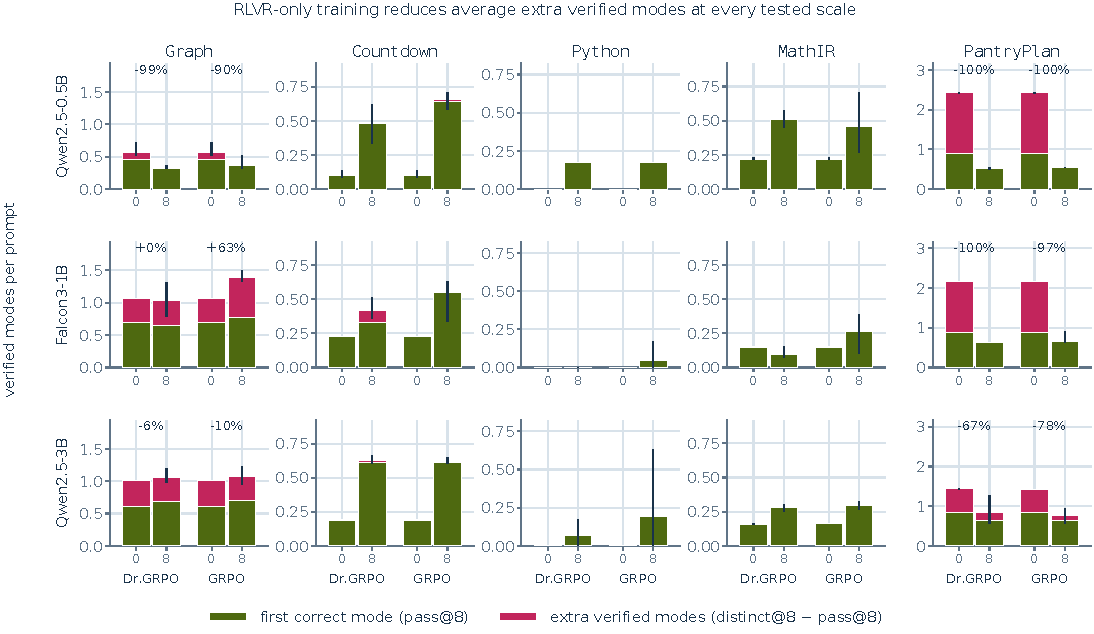
\includegraphics[width=\linewidth]{figures/baseline_collapse_precheck.pdf}
  \caption{\textbf{Both verifier-only objectives reduce verified solution
  breadth, at every scale.} Bars split \texttt{distinct@8} into the first correct
  mode and every verified mode beyond it, at training pass 0 and pass 8, for
  unmodified Dr.GRPO then GRPO in each panel. All 150 evaluations are complete at five
  seeds and four fixed \(K=8\) draws; whiskers are the seed range and pass 0 is
  measured per method. Badges give the change in extra verified modes, printed only
  where pass-0 breadth exceeds \(.05\) of them; the other three domains start at
  \(.011\) or less.
  \label{fig:baseline-precheck}}
\end{figure}

\begin{table}[h]
  \centering
  \caption{\textbf{Problem precheck, five-domain macro-averages.} Both
  verifier-only objectives at pass 0 and pass 8, all three scales, five seeds
  and four fixed $K=8$ draws per model--domain--method comparison. ``Extra modes'' is
  \texttt{distinct@8}$-$\texttt{pass@8}; ``removed'' is the fraction of that
  quantity lost between pass 0 and pass 8. Breadth loss is present at every
  scale and is far from uniform across scales, and at Falcon3-1B Dr.GRPO
  macro \texttt{pass@8} falls as well.}
  \label{tab:baseline-collapse-precheck}
  \small
  \setlength{\tabcolsep}{4.5pt}
  \begin{tabular}{@{}l*{6}{c}@{}}
    \toprule
    & \multicolumn{3}{c}{\textbf{Dr.GRPO}} & \multicolumn{3}{c}{\textbf{GRPO}} \\
    \cmidrule(lr){2-4}\cmidrule(l){5-7}
    \textbf{Model} & \texttt{pass@8} & extra modes & removed
                   & \texttt{pass@8} & extra modes & removed \\
    \midrule
    Qwen2.5-0.5B & \(0.335 \to 0.402\) & \(0.329 \to 0.002\) & 99.4\% & \(0.335 \to 0.435\) & \(0.329 \to 0.006\) & 98.2\% \\
Falcon3-1B & \(0.391 \to 0.342\) & \(0.332 \to 0.094\) & 71.6\% & \(0.391 \to 0.454\) & \(0.332 \to 0.135\) & 59.4\% \\
Qwen2.5-3B & \(0.356 \to 0.455\) & \(0.205 \to 0.120\) & 41.5\% & \(0.356 \to 0.490\) & \(0.199 \to 0.101\) & 49.4\% \\
\bottomrule

  \end{tabular}
\end{table}


Graph and PantryPlan contain substantial initial breadth at every scale;
the other three domains begin with at most $.011$ extra modes per prompt.
A retained-breadth percentage is therefore reported only when the initial
extra-mode count exceeds $.05$. Raw $\texttt{distinct@8}$ ends below its
initial value in six of the 15 Dr.GRPO domains. ReplayDr.GRPO does so in
two available domain summaries, both PantryPlan; Falcon Countdown uses
four admissible seeds. These observations concern sampled held-out support,
not the survival histories of particular stored modes.

Uniform-action references are meaningful for the enumerable Graph and
Pantry representations. They are not defined for open-ended programs or
derivations. Pantry's bit-uniform reference exceeds every final model, so
this domain is a support-concentration stress test rather than evidence
of complete support coverage.

\begin{table}[t]
  \centering
  \caption{\textbf{Absolute references for raw \texttt{distinct@8}.}
  \emph{Uniform} samples the exposed action representation uniformly and is
  defined only for Graph (27 color strings) and PantryPlan (64 bit masks).
  Frozen is the matched pass-0 model; the final two columns are pass-8 means.
  Dashes avoid pretending that an open-ended program or derivation space has a
  canonical uniform distribution.}
  \label{tab:absolute-support-references}
  \scriptsize
  \setlength{\tabcolsep}{4.2pt}
  \begin{tabular}{@{}llrrrr@{}}
    \toprule
    \textbf{Model} & \textbf{Domain} & \textbf{Uniform} & \textbf{Frozen}
      & \textbf{Dr.GRPO} & \textbf{ReplayDr.GRPO} \\
    \midrule
        \qwenmark{}2.5-0.5B & \texttt{Graph} & 1.633 & .561 & .325 & 2.438 \\
     & \texttt{PantryPlan} & 2.153 & 2.426 & .522 & 1.539 \\
    \addlinespace[2pt]
    Falcon3-1B & \texttt{Graph} & 1.633 & 1.070 & 1.034 & 1.717 \\
     & \texttt{PantryPlan} & 2.153 & 2.162 & .633 & 1.576 \\
    \addlinespace[2pt]
    \qwenmark{}2.5-3B & \texttt{Graph} & 1.633 & 1.012 & 1.060 & 1.637 \\
     & \texttt{PantryPlan} & 2.153 & 1.445 & .841 & 1.514 \\
    \bottomrule

  \end{tabular}
\end{table}


\subsection{Fresh-gradient degeneracy and observed output collapse}
\label{app:degenerate-groups}

A Dr.GRPO group with identical rewards has exactly zero fresh task gradient.
Only mixed groups containing both correct and incorrect responses can
supply fresh reward information; optimizer momentum can still move a
policy when that task gradient is zero. The fractions of mixed groups
over all 3,072 Qwen2.5-0.5B updates, averaged over five seeds, are:

\begin{center}
\small
\begin{tabular}{@{}lrr@{}}
\toprule
\textbf{Domain} & \textbf{Dr.GRPO} & \textbf{ReplayDr.GRPO} \\
\midrule
Graph coloring & .144 & .954 \\
Countdown & .140 & .456 \\
Python factors & .015 & .185 \\
MathIR & .364 & .453 \\
PantryPlan & .123 & .789 \\
\bottomrule
\end{tabular}
\end{center}

Thus 98.5\% of Python control updates carry zero fresh task gradient.
Replay supplies a verified-likelihood gradient directly and can also
change the policy so that later fresh groups become mixed.

A raw-response audit of all five Qwen2.5-0.5B Python control seeds establishes
observed output collapse directly. At pass 0, a draw has 7.99 unique raw
completions per prompt on average. By steps 288--480, every seed produces
32 byte-identical temperature-1 samples per prompt, also identical to the
logged greedy completion, on all 128 prompts. This persists through step
3,072. Terminal draws contain 1.00 unique completion per prompt in the
control and 1.97 under replay. A collapsed completion can be incorrect:
this is one observed completion per prompt, not one correct key everywhere.
Aggregate endpoint equality or zero draw spread alone would not establish
that conclusion, nor does this finite audit rule out low-probability tails.

These checks explain a vulnerability of the registered sparse binary-reward
recipe. They do not establish dominance over methods that keep fresh
on-policy signal active. Dynamic mixed-group sampling, larger groups,
reference KL, token-entropy regularization, and wider-decoding evaluations
remain relevant controls beyond the registered factorial.

\subsection{Fixed-bank exemplar score trajectories}
\label{app:fixed-bank-survival}

The fixed-bank study tracks Qwen2.5-0.5B ReplayDr.GRPO on Graph for seeds
43--47. Before step 384's fresh group, bank membership and fresh counts
are frozen; admission then stops while uniform replay continues through
3,072 updates under the same training recipe. Every frozen exemplar is
identified by prompt and canonical-key fingerprints, without selection by
its score trajectory. Each scheduled replay visit records mean token log
probability $s$ and sequence log probability $\ell$. Changes compare an
identity's first and final post-freeze visits; observation steps can differ
across identities.

All 3,406 frozen identities across 1,575 seed--prompt pairs have finite,
aligned scores at every scheduled visit: 8--9 visits per identity and
29,041 observations in total. The pooled median change is $+.038$
nat/token (95\% interval $[+.025,+.048]$), but the 10th percentile is
$-.256$ and $2.61\%$ of identities lose more than $.5$ nat/token
($[1.54,3.77]\%$). The worst intermediate change is $-1.328$ nat/token.
On the sequence scale, the median is $+.154$ nat/sequence
($[+.104,+.198]$), while $21.99\%$ lose more than $.5$ nat/sequence.
Lengths range from 4 to 100 tokens, so the two threshold percentages have
different meanings.

\begin{figure}[H]
  \centering
  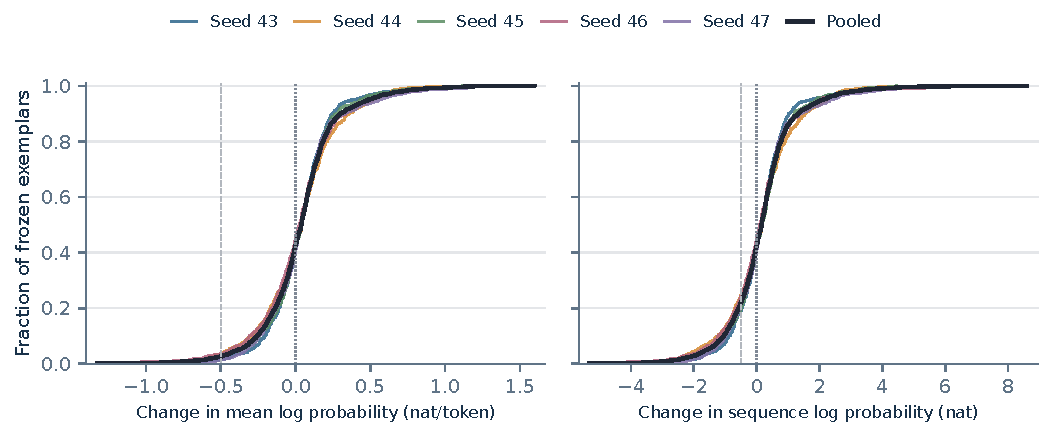
\includegraphics[width=.95\linewidth]{figures/e121_fixed_bank_survival.pdf}
  \caption{\textbf{Fixed-exemplar scores improve centrally but retain a declining tail.}
  Empirical cumulative distributions show first-to-final post-freeze score
  changes for every frozen identity, with one curve per seed and the pooled
  identity distribution. Mean token and sequence scores are separate panels;
  positive values indicate increased teacher-forced likelihood. Neither panel
  measures the exact probability of generating a canonical mode during policy sampling.}
  \label{fig:e121-fixed-bank-survival}
\end{figure}


Pooled summaries weight identities equally. Descriptive 95\% intervals
use 10,000 hierarchical bootstrap draws (random seed 121), resampling prompts within each
original seed and then five seeds with replacement; repeated seeds reuse
their within-draw prompt sample. Linear empirical quantiles and percentile
intervals are analysis choices. The artifact
\path{paper/results/e121_fixed_bank_survival.json} retains all seed summaries,
identity trajectories, source hashes, and audit diagnostics.

These are teacher-forced score surrogates, not exact probabilities of
sampling canonical modes. Visits do not cover every intervening update,
and the declining tails exclude a claim that every exemplar improves.
Without a matched no-replay fixed-bank arm, this study does not identify
a causal replay effect. It neither numerically validates
Theorem~\ref{thm:replay-retention}'s probability floor nor certifies a finite-network
guarantee. It adds longitudinal measurements of fixed exemplars to the
held-out support evidence.
